\section{background and related work}
	% -related work
	% 	-LOS vs NLOS (SNR實驗)
	% 	-communication not only localization
	% 	-luxapose
	% -rolling shutter相關知識
	% 	-operation and channel model
	% 	-特色:跟perspective, orientation無關

\subsection{Camera-received VLC}
\subsubsection{Screen-to-camera communications}
A number of prior works~\cite{perli2010pixnet,hao2012cobra,hu2013lightsync} utilized cameras as the receiver to implement one-way communication links. Those works utilized a LCD screen as the transmitter. The main benefit of this approach is that both the ability to display different colors and the high resolution of the LCD could be fully exploited, to improve the data rate.

PixNet \cite{perli2010pixnet} utilized the large quantity of pixels on a LCD to form OFDM symbols to transmit data to the camera receiver, and the implemented prototype has perspective correction ability.

COBRA \cite{hao2012cobra} proposed a similar approach that uses pixels as as barcodes and utilized the color information of pixels to achieve higher signal to noise ratio.
These works, however, did not solve the problems raised by the unsynchronized transmitter and receiver pair. The presented solution is to repeat the same packet transmission twice in order to guarantee the reception of all signal segments.

LightSync \cite{hu2013lightsync} introduces inter-frame erasure coding and line sequence number to reduce the high packet error rate due to synchronization issues. The approach also actively filters out rolling-shutter effects.

VRCodes (NewsFlash) \cite{vrcodes} takes advantage of the rolling shutter effect to decode visual tags displayed on LCDs. The tags use multiple pixels of different colors, modulated at up to 120Hz to transmit data. The technology exploits the "flicker-fusion threshold" of the human eye to blend the tags into the background by rapidly flashing complimentary hues of color, still visible to a rolling shutter camera. This work suggests how different color channels could be used to increase data throughput, while still keeping transmissions imperceptible to humans.

Visual MIMO \cite{visualmimo1, visualmimo2, visualmimo3} is a method that uses any light-emitting spatial array as the transmitter and uses ordinary cameras as the receivers.
It proposes a photometric modeling for hidden imagery and can realize a dual use of the electronic display: to display an image for human observation while simultaneously transmitting hidden bits for decoding by a camera.

Compared to these works, we proposed to use only a single LED light as the transmitter and a commonly available CMOS camera as the receiver, and many design considerations are not the same as these prior research works utilizing multiple optical transmitting sources.


\subsubsection{Single-LED-to-camera communications}
Three works \cite{roberts2013undersampled, danakis2012using,landmark} have previously investigated how to implement single-LED-to-camera communication links. 
In~\cite{roberts2013undersampled}, the author proposes undersampled frequency shift OOK (UFSOOK), which allows the use of a high signal frequency while the modulation can still be decoded by a common camera with 30 fps (frame rate per second). The scheme is compatible to both global shutter and rolling shutter cameras, but the maximum achievable data rate is only half of the frame rate per light source.

In \cite{danakis2012using}, the authors utilized rolling shutter sampling to encode data with Manchester coding at high symbol rate, and was the first work to take advantage of the rolling shutter to implement CamCom. 
However, the implementation exhibits a high packet drop rate due to the long processing time of the decoder application per frame and lack of considerations for synchronization issues. Thus, the reception is not continuous and some frames are inevitably lost. The transmitter then needs to send signal.
In addition, the transmitting light needs to illuminate the entire image for the receiver to demodulate the transmission.We can achieve a data rate much higher than 50\% of the frame rate per light source, and have designs to address the issues caused by the exposure operation of the camera and unsynchronized nature of the communication link.
A further drawback in this work is that the modulated signal can produce a human perceivable flicker from transmitting LED. The authors alleviate this by imposing a DC bias on the signal, which in turn decreases its dynamic range and SNR at the receiver. This makes the scheme require significantly brighter lights and more complex driving hardware than our proposed approach.

In \cite{landmark}, the author used binary frequency shift keying (BFSK) of a high frequency PWM signal to encode data that can be used as localization landmarks. On the receiver side, they exploited rolling shutter camera sensors to detect high-frequency changes in the intensity of light reflected off surfaces, which is indirect line-of-sight of the camera. The data rate is only 1.25 bytes per second (the authors claimed that it is fast enough to send an ID code) while in our work there is a need to increase the data rate to communicate rather than just perform localization. To detect the transmitting frequency, they used 1-D fast Fourier transform. However, we have tried the FFT method before and it usually requires a threshold to eliminate the noise. It is hard to have a general threshold which can be adopted in different environments. For the receiver which is unsynchronized with the transmitter, they proposed a sliding window approach where they first stitch all of the captured frames together into a single, long image. Then they can detect the frequency by sliding the window and locating the window position corresponding to the highest power. However, we can stitch the images only if the light is full of whole image (for example, reflected from the surface). Moreover, if there is a symbol loss between the two frames, then the result of stitching images would likely be inaccurate. In our work, we use additional schemes to address these problems.


\subsection{Channel Model of Rolling Shutter Camera}
\begin{figure}[!htb]
	\centering
	\begin{subfigure}[h]{0.3\textwidth}
		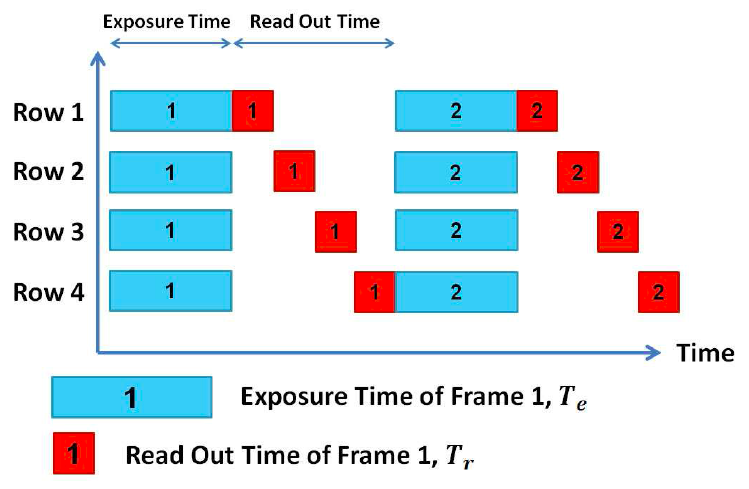
\includegraphics[width=\textwidth]{fig/global_shutter.png}
		\caption{Global Shutter Operation}
	\end{subfigure}
	~
	\begin{subfigure}[h]{0.1\textwidth}
		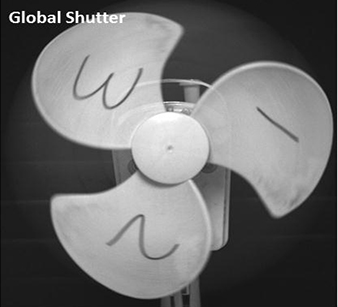
\includegraphics[width=\textwidth]{fig/fan_global}
		\caption{Global Shutter Example}
	\end{subfigure}
	\\
	\begin{subfigure}[h]{0.3\textwidth}
		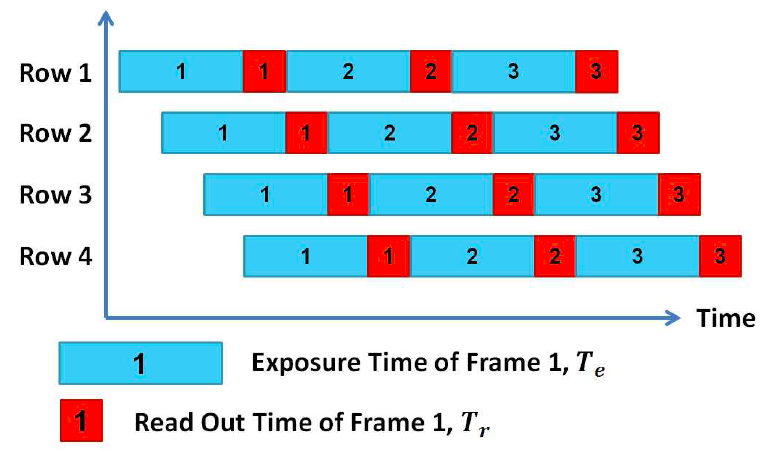
\includegraphics[width=\textwidth]{fig/rolling_shutter.png}
		\caption{Rolling Shutter Operation}
	\end{subfigure}
	~
	\begin{subfigure}[h]{0.1\textwidth}
		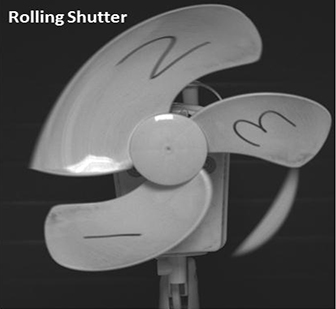
\includegraphics[width=\textwidth]{fig/fan_rolling}
		\caption{Rolling Shutter Example}
	\end{subfigure}
\caption{Shutter mechanisms}
\label{fig:compare_shutter}
\end{figure}

\subsubsection{Rolling Shutter Operation}
\autoref{fig:compare_shutter} compares global and rolling shutter operation \cite{imagesensor}. Global shutters, which are commonly implemented on CCD sensors, expose all pixels on the sensor simultaneously and gather incoming light over all pixels during the exposure time. 
Although some CMOS sensors use a global shutter, the majority found in the consumer market utilize a rolling shutter. 
One of the key properties of a rolling shutter camera sensor is its sequential read-out architecture. 
As in most CMOS sensors there is no per pixel storage to hold the accumulated charge during the exposure operation, the exposure period happens right before each read-out operation. 
The read-out architecture can process charge voltage signals one row at a time. 
Since the read-out durations of two rows cannot overlap, each of the exposure durations of a row of pixels is shifted by a fixed amount of read-out time (represented by $T_r$ in \autoref{fig:RollingShutter}), resulting in the so-called rolling shutter operation.
For each pixel, the incoming intensity modulated signal is integrated for a time period called exposure time (represented by $T_e$ in \autoref{fig:RollingShutter}). 

\begin{figure}[!htb]
	%\centering
	%\hspace{5em}
	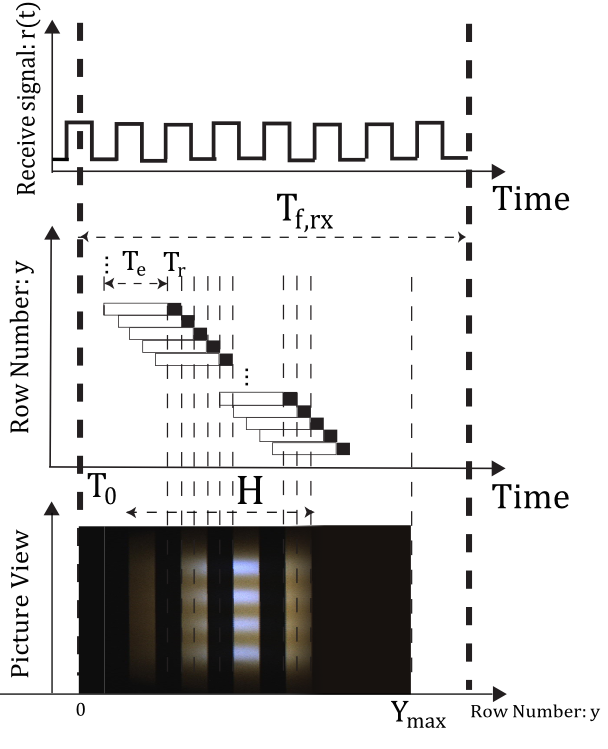
\includegraphics[scale=0.35]{fig/RollingShutter2}
	\caption{The receiving operation of a rolling shutter camera sensor. Top: the original received signal; middle: the exposure and read-out processes; bottom: the resulted image. $T_{f,rx}$: receiving frame duration; $T_e$: exposure time; $T_r$: read-out time.}
	\label{fig:RollingShutter}
\end{figure}

\autoref{fig:RollingShutter} shows the receiving operation of a rolling shutter camera sensor to an intensity modulated signal.
Assume the original received signal in time is given by $r(t)$, which includes the signal from the transmitted light and other ambient interference. Considering the direct integration operation taking place during exposure and the rolling shutter operation, the intensity of a pixel in $y$-th row in the image, $I[y]$, which also represents the total amount of photons received by the pixel during exposure, is given by:

\begin{equation}
	I[y]=\int^{T_0+y T_r+T_e}_{T_0+y T_r} r(t) dt, \; 0 \leq y \leq Y_{\max},
	\label{eq:rollingshutter}
\end{equation}

where $T_r$ is the read-out time, $T_e$ is the exposure time, $T_0$ is a reference time point that corresponds to the start of the exposure time of the first row of pixels in the image, and $Y_{\max}$ is the number of rows of pixels in the image. Note that the transmitting light might not illuminate all rows in the image. In that case, the transmitted signal is only observed in $I[Y_{\operatorname{top}} \leq y \leq Y_{\operatorname{top}}+H]$, where $H$ represents the height of the image area illuminated by the transmitting light.

The direct integration operation can be considered as a low-pass filter (or a moving average filter), and thus $I[y], 0 \leq y \leq Y_{\max}$ is a filtered version of the original received signal $r(t)$. The filter distorts high frequency components in the received signal, especially the ones with a frequency higher than $1/T_e$.

\subsubsection{Time Gap in the Frame Duration}
Utilizing \autoref{eq:rollingshutter}, if the transmitting light occupies all rows of pixels in the image, the end of exposure of the last row in this image frame is $T_0 + Y_{\max} T_r + T_e$, while the start of exposure of the first row in the next image frame is $T_0 + T_{f,rx}$. The \textbf{time gap} between these two events $T_{f,rx} - Y_{\max} T_r - T_e$, when $T_e$ is small, is significant for most cameras.
This is the amount of time during which the camera is not performing any exposure operation, i.e., not receiving the transmitted signal. Signal transmitted during this time period is lost. \autoref{tab:readout} summarizes both the values of this time gap (without subtracting the exposure time $T_e$) and the percentage of time contributed by this time gap compared to a frame duration. Note that for some cameras, this could be up to half of the receiving frame duration. In addition, in the case that the transmitting light does not illuminate all rows in the image, this time gap could further increase.


\begin{table*}[!htb]
\centering
\caption{Summary of Camera Parameters}
   \tabcolsep=0.08cm
    \begin{tabular}{c|c|c|c|c}
    \hline
                    % & Image Resolution & Frame Rate & Measured & Time Gap (ms)    \\
                    % &   ($X_{\max}$ x $Y_{\max}$)                &  (fps)          &  Read-out &  (Percentage of       \\ 
                    % &  &  & Time ($\mu$s) &  Frame Duration)   \\ 
	    & Image Resolution & Frame Rate & Measured Read-out & Time Gap (ms)    \\
	    &   ($X_{\max}$ x $Y_{\max}$)                &  (fps)          & Time ($\mu$s) &  (Percentage of       \\ 
	    &  &  &  &  Frame Duration)   \\    
    \hline \hline
    Point Grey Flea3 & 2048x1080          & 30         & 14.75                   & 17.40 (52.23\%) \\ \hline
    Apple iPhone 5S  & 1920x1080          & 29.98      & 19.15                   & 12.67 (37.99\%) \\ \hline
    Apple iPhone 4S  & 1920x1080          & 29.87      & 24.48                   & 7.04 (21.03\%) \\ \hline
   HTC New One      & 1920x1080          & 30         & 18.79                   & 13.04 (39.11\%) \\ \hline
    Apple iPhone 4   & 1280x720           & 29.97      & 44.88                   & 1.05 (3.15\%)  \\ \hline
    HTC Desire HD    & 800x480            & 29.08      & 55.18                   & 7.90 (22.97\%) \\ \hline
    Google Nexus One & 720x480            & 30.57      & 59.66                   & 4.07 (12.45\%) \\ \hline
    \end{tabular}
    \label{tab:readout}
\end{table*}


\subsubsection{Channel Characteristics}
In summary, the single-LED-to-rolling-shutter-camera channel exhibits two major characteristics:
\begin{enumerate}
	\item The signal that can be obtained from the image is a low-pass filtered version of the original received signal in time. The filter create distortions in high frequency components.
	\item The receiving process is not continuous. This can be considered as a form of channel fading; when it takes place, the channel loss is infinite. The ratio of signal lost is determined by a constant time gap that depends on camera parameters, and the size of the image area illuminated by the transmitting light. A smaller image area corresponds to a higher ratio of signal lost.
\end{enumerate}



